% ============================================================
% CWI 2026 poster visuals - TikZ source (FIXED 2026-08-16)
% Fixes vs the 2026-08-16 draft notes:
%  F1: "line width=pt" (invalid LaTeX) -> 0.4pt / 0.8pt   [x4]
%  F2: figure caption "Shor [[1]" -> "Shor [[9,1,3]]"
%  F3: \pgfmathtruncatemacro{\angle}{...} redefined \angle -> \ang
% ============================================================

% ---- Figure 1 (Panel 1): Continuous vs. staircase fidelity ----
\documentclass[border=2pt]{standalone}
\usepackage{tikz}
\usepackage{pgfplots}
\pgfplotsset{compat=1.18}

\begin{document}
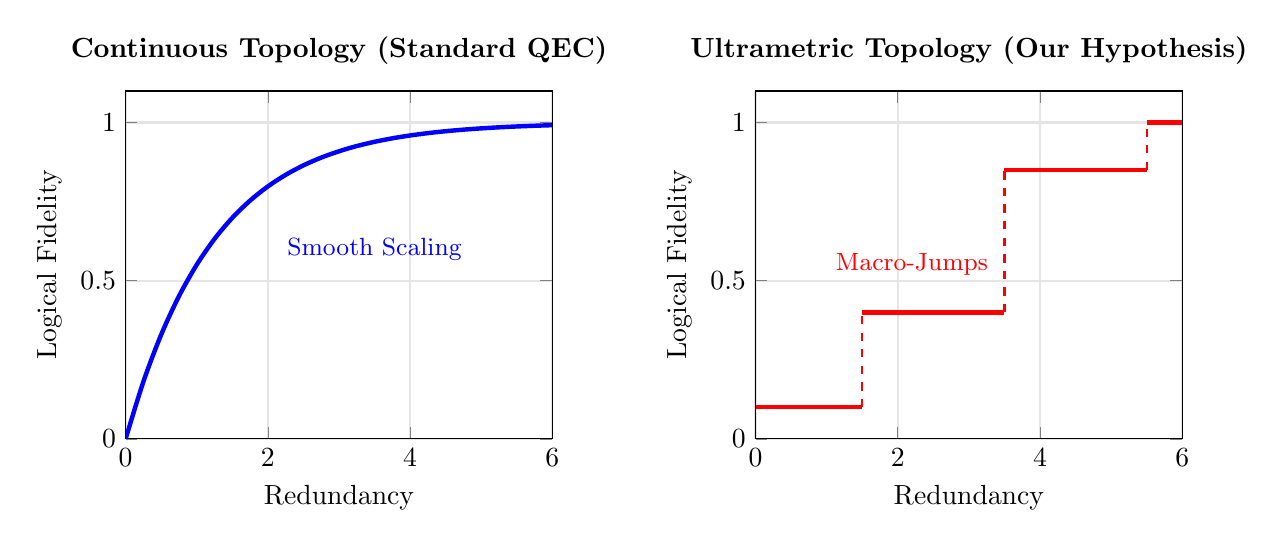
\begin{tikzpicture}

  % Left Plot: Continuous Topology (Standard QEC)
  \begin{scope}[shift={(0,0)}]
    \begin{axis}[
        title={\textbf{Continuous Topology (Standard QEC)}},
        xlabel={Redundancy},
        ylabel={Logical Fidelity},
        xmin=0, xmax=6,
        ymin=0, ymax=1.1,
        xtick={0,2,4,6},
        ytick={0,0.5,1},
        grid=both,
        grid style={line width=0.4pt, draw=gray!10},
        major grid style={line width=0.8pt, draw=gray!20},
        width=7cm, height=6cm
    ]
      \addplot[smooth, blue, ultra thick, domain=0:6] {1 - exp(-0.8*x)};
      \node[blue, font=\small] at (axis cs:3.5,0.6) {Smooth Scaling};
    \end{axis}
  \end{scope}

  % Right Plot: Ultrametric Topology (Hypothesis)
  \begin{scope}[shift={(8,0)}]
    \begin{axis}[
        title={\textbf{Ultrametric Topology (Our Hypothesis)}},
        xlabel={Redundancy},
        ylabel={Logical Fidelity},
        xmin=0, xmax=6,
        ymin=0, ymax=1.1,
        xtick={0,2,4,6},
        ytick={0,0.5,1},
        grid=both,
        grid style={line width=0.4pt, draw=gray!10},
        major grid style={line width=0.8pt, draw=gray!20},
        width=7cm, height=6cm
    ]
      % Staircase steps
      \addplot[ultra thick, red] coordinates {(0,0.1) (1.5,0.1)};
      \addplot[ultra thick, red] coordinates {(1.5,0.4) (3.5,0.4)};
      \addplot[ultra thick, red] coordinates {(3.5,0.85) (5.5,0.85)};
      \addplot[ultra thick, red] coordinates {(5.5,1.0) (6.0,1.0)};

      % Dashed connector lines for jumps
      \draw[dashed, red, thick] (axis cs:1.5,0.1) -- (axis cs:1.5,0.4);
      \draw[dashed, red, thick] (axis cs:3.5,0.4) -- (axis cs:3.5,0.85);
      \draw[dashed, red, thick] (axis cs:5.5,0.85) -- (axis cs:5.5,1.0);

      \node[red, font=\small] at (axis cs:2.2,0.55) {Macro-Jumps};
    \end{axis}
  \end{scope}

\end{tikzpicture}
\end{document}

% ---- Figure 2 (Panel 2): Hierarchical environmental nesting ----
\documentclass[border=2pt]{standalone}
\usepackage{tikz}

\begin{document}
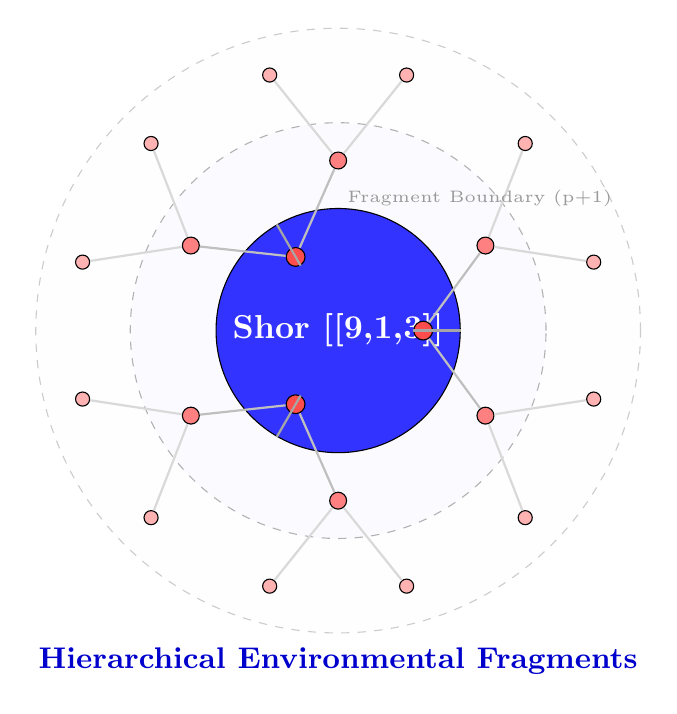
\begin{tikzpicture}[scale=1.2, every node/.style={transform shape}]

  % Concentric Hierarchical Boundaries
  \draw[dashed, gray!40, fill=blue!5,  fill opacity=0.1] (0,0) circle (3.2cm);
  \draw[dashed, gray!60, fill=blue!10, fill opacity=0.1] (0,0) circle (2.2cm);
  \draw[dashed, gray!80, fill=blue!15, fill opacity=0.1] (0,0) circle (1.2cm);

  % Central Logical Hub (Shor Code Node)
  \node[circle, draw=black, fill=blue!80, text=white, font=\bfseries, inner sep=4pt] (Shor) at (0,0) {Shor [[9,1,3]]};

  % Tier 1 Environment Qubits (Inner Ring)
  \foreach \a in {0, 120, 240} {
    \node[circle, draw=black, fill=red!70, inner sep=2pt] (E1-\a) at (\a:0.9cm) {};
    \draw[thick, gray!70] (Shor) -- (E1-\a);
  }

  % Tier 2 Environment Qubits (Middle Ring branching off Tier 1)
  \foreach \a in {0, 120, 240} {
    \foreach \b in {-30, 30} {
      \pgfmathtruncatemacro{\ang}{\a + \b}
      \node[circle, draw=black, fill=red!50, inner sep=1.8pt] (E2-\ang) at (\ang:1.8cm) {};
      \draw[thick, gray!50] (E1-\a) -- (E2-\ang);
    }
  }

  % Tier 3 Environment Qubits (Outer Ring branching off Tier 2)
  \foreach \a in {0, 120, 240} {
    \foreach \b in {-30, 30} {
      \foreach \c in {-15, 15} {
        \pgfmathtruncatemacro{\ang}{\a + \b + \c}
        \node[circle, draw=black, fill=red!30, inner sep=1.5pt] (E3-\ang) at (\ang:2.8cm) {};
        \pgfmathtruncatemacro{\parent}{\a + \b}
        \draw[thick, gray!30] (E2-\parent) -- (E3-\ang);
      }
    }
  }

  % Labels and Visual Anchors
  \node[font=\small\bfseries, text=blue!80!black] at (0,-3.5) {Hierarchical Environmental Fragments};
  \node[font=\tiny, text=gray!80] at (1.5, 1.4) {Fragment Boundary (p+1)};

\end{tikzpicture}
\end{document}

% ---- Figure captions for the poster (FIXED F2) ----
% Figure 1 (Panel 1): "Comparison of logical fidelity scaling. Left: standard continuous
%   topology — fidelity scales smoothly with qubit count. Right: hypothesized ultrametric
%   staircase — flat plateaus and sharp macro-jumps across p-adic boundaries. Hypothesis
%   only; not observed."
% Figure 2 (Panel 2): "Radial map of the Shor [[9,1,3]] code embedded in a hierarchical
%   environmental matrix. Shaded boundary zones isolate discrete interaction fragments
%   structured along the branching tree network."
